\documentclass[22pt]{beamer}
\usepackage{textcomp}
\usepackage[orientation=portrait, size=custom, width=91.44, height=91.44,scale=1.3]{beamerposter} % 36in*2.5 = 90cm
\usepackage[absolute,overlay]{textpos}
\usepackage{bookmark} %pdflatex says to use this to avoid errors...
\usepackage{graphicx} %for including images
\graphicspath{{figs/}} %location of images
\usepackage{wrapfig} %wrap text around the images
\usepackage{listingsutf8}    
\usepackage{amsmath}
\usepackage{gensymb}
\usepackage[export]{adjustbox}
\usepackage[skins,theorems]{tcolorbox}
\usepackage{tikz}
\newcommand*\circled[1]{\tikz[baseline=(char.base)]{
            \node[shape=circle,draw,inner sep=2pt] (char) {#1};}}
\usepackage{array}
\usepackage{booktabs,adjustbox}
\usepackage{subcaption} 


\usetheme{Berlin}
\definecolor{MacBlue}{rgb}{0.10196,0.22353,0.53725}
\definecolor{MacMaroon} {rgb}{0.47843, 0, 0.23137}
\definecolor{MacMaroon2} {rgb}{0.47451, 0, 0}
\definecolor{MacGray}{rgb}{0.50196,0.49804,0.51765}
\definecolor{MacMaroon3}{rgb}{00.47,0.2,0.31}
\definecolor{MacGold}{rgb}{1, 0.75,0.35}
\usecolortheme[named=MacBlue]{structure}
\setbeamertemplate{caption}[numbered]
\setbeamertemplate{navigation symbols}{}

\title{Approximate Regular Expressions: A Comparison of Exact and Approximate Matching Algorithms}
\subtitle{}  
  \author[Gadriwala, Noshin \& Siddiqui]{Umme Salma Gadriwala, Tasnim Noshin, Rumsha Siddiqui \vspace{0.3cm} \newline \small \{gadriway, noshint, siddiqur\}@mcmaster.ca}
  \institute[McMaster University]{Department of Computing and Software, McMaster University

1280 Main St. W, Hamilton, Ontario, Canada L8S 4L8}
  \date{April 2019}

\begin{document}
\begin{frame}[fragile]

\begin{textblock}{2}(0.7,1)

\includegraphics[height=8.5cm]{englogo.png}
\end{textblock}

\begin{textblock}{8}(4,1)
\titlepage
\end{textblock}

\begin{textblock}{2}(12.7,0.75)

\includegraphics[height=12cm]{cslogo.png}
%\centering
%\textbf{Tweet us} \\
%your thoughts: \\
%{[worth pursuing?] [achievable?]}
%{\color{MacBlue} @TeamDeepCheck \#MacCSCapstone \#MacEng}
\end{textblock}

\begin{textblock}{7.25}(0.5,3.1)

\begin{block}{Motivation}
-different applications

\end{block}

\begin{block}{Problem}
-when to use
-can only implement approx?
\end{block}

\begin{block}{Solution}
Implement algorithm and explore efficiency of Thompson's and Millers and Myers
\end{block}


\begin{block}{Background Study}
\textbf{Exact Matching}:

\begin{figure}
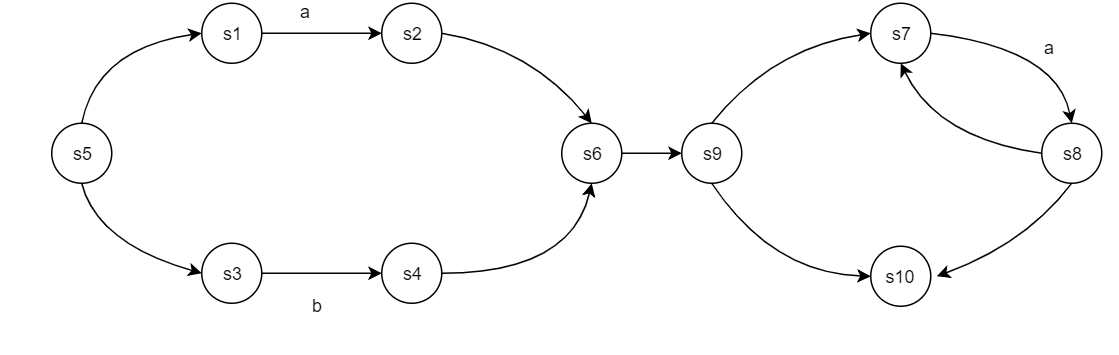
\includegraphics[scale=1.5]{ThompsonsNFA.PNG}
\end{figure}

\vspace{5mm} %5mm vertical space



\textbf{Approximate Matching}:


\begin{figure}
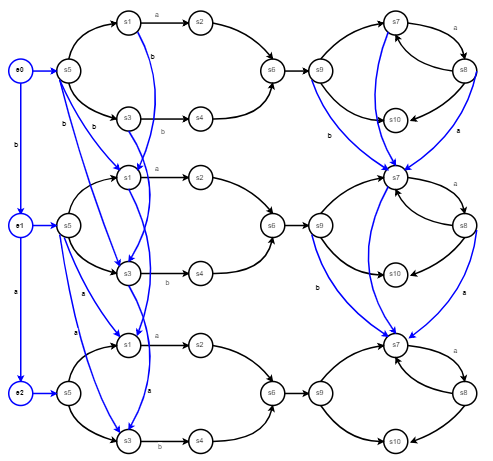
\includegraphics[scale=2]{MillerAndMyersAlgorithm.PNG}
\end{figure}

\end{block}
\end{textblock}


\begin{textblock}{7.25}(8.25,3.1)
\begin{block}{Methodology}

explain what doing

graph

\end{block}


\begin{block}{Conclusions \& Future Work}
final result

future:other algos
\end{block}


\begin{block}{Acknowledgements}
We thank Dr. Sekerinski for inspiring this project, as well as his continued guidance in our learning and endeavours. We also thank Spencer Park and Erin Varey for their invaluable feedback and support. 
\end{block}

%--------------------------------------------
%REFERENCES
\begin{block}{References}
\setbeamertemplate{bibliography item}{\insertbiblabel}
\bibliographystyle{ieeetr}
{\scriptsize
\bibliography{bib}}
\end{block}

\begin{comment}
\begin{block}{References}
\setbeamertemplate{bibliography item}{\insertbiblabel}
\bibliographystyle{ieeetr}
{\scriptsize
\bibliography{bib}}
\end{block}
\vspace{-1.8mm}
\end{comment}
\end{textblock}

%
%\begin{textblock}{7.5}(0.5,14.6)
%\centering
%\textbf{Tweet us} \\
%your thoughts on DeepCheck and where you think the future of neural networks is headed \\
%{\color{MacBlue} @TeamDeepCheck \#MacCSCapstone \#MacEng}
%
%\end{textblock}

\end{frame}
\end{document}
